\subthesischapter{Escenarios de entrenamiento}
La creación de las escenas es dinámica, pues se adapta a los valores de modalidad y parámetros seleccionados en la configuración del juego. Estos valores son fundamentales, ya que determinan el funcionamiento y por ende la experiencia de juego. Para llevar a cabo dicha tarea, fue necesario implementar un script llamado WorldCreator.cs.

WorldCreator.cs es el núcleo de nuestra creación escénica. Este script se encarga de construir la totalidad del entorno del juego. El método Awake() en el script WorldCreator cumple una función fundamental en la inicialización y preparación del escenario de juego. En primer lugar, verifica la integridad del objeto trackPrefab, asegurándose de que no sea nulo mediante una aserción (Assert). Este objeto representa la pista sobre la cual se construirá el mundo del juego. A continuación, se procede a la creación dinámica del terreno (Terrain) del juego. Se genera un nuevo objeto de datos de terreno (TerrainData) y se asigna al terreno recién creado. Además, en el método se calcula y almacena las dimensiones del objeto de la pista (trackPrefab) utilizando el componente MeshFilter. Estas dimensiones se utilizan posteriormente para posicionar los árboles y otros elementos de manera coherente respecto a la pista, garantizando la cohesión visual del mundo del juego. Por último, el método Awake() asigna el material (terrainMaterial) al terreno, definiendo así la apariencia visual del paisaje. Este proceso sienta las bases para el entorno tridimensional en el cual se desarrollará la acción del juego.

\begin{figure}[ht]
    \centering
    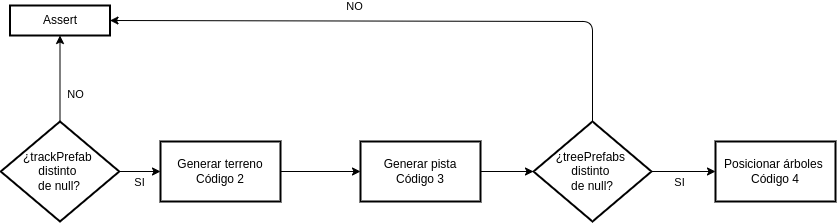
\includegraphics[scale=0.5]{images/generate-world.png}
    \caption{Flujo para la creación del entorno de juego}
    \label{fig: generate-world}
\end{figure}

\begin{center}
\begin{minipage}{0.8\textwidth}
\begin{lstlisting}[language=c, caption={Generar terreno},label={hola}]
 //Obtener el terreno activo en la escena
 terrain = Terrain.activeTerrain;
 
 // Crear un nuevo objeto de datos del terreno
 var data = new TerrainData();

 terrain = Terrain.CreateTerrainGameObject(data).GetComponent<Terrain>();
 
 // Establecer la posición del terreno en el origen del mundo
 terrain.transform.position = Vector3.zero;     

 // Obtener los límites del objeto de pista  mediante su componente MeshFilter           
 var bounds = trackPrefab.GetComponent<MeshFilter>().sharedMesh.bounds;
 trackSize = bounds.size;
 
 // Asignar material al terreno generado
 terrain.materialTemplate = terrainMaterial;
\end{lstlisting}
\end{minipage}  
\end{center}

\begin{center}
\begin{minipage}{0.8\textwidth}
\begin{lstlisting}[language=c, caption={Generar pista}]
 float zMin = chunkIndex * chunkSize;
 float zMax = zMin + chunkSize;
 terrain.terrainData.size = new Vector3(chunkSize, maxHeight, zMax);

 var track = Instantiate(
                 trackPrefab, 
                 new Vector3(chunkSize*0.5f, 0.0f, zMin), 
                 Quaternion.identity
             ).transform;

 track.localScale = new Vector3(1.0f, 1.0f, chunkSize / trackSize.z);
\end{lstlisting}
\end{minipage}  
\end{center}

\begin{center}
\begin{minipage}{0.8\textwidth}
\begin{lstlisting}[language=c, caption={Posicionar árboles}]    
 for (int i = 0; i < treeDensity; i++) {
    float side = Random.value > 0.5f ? 1.0f : 0.0f;

    // Generar coordenadas aleatorias dentro del rango especificado
    float z = Random.Range(zMin, zMax);  

    float x = Random.Range(0, chunkSize * 0.5f - trackSize.x * 0.5f) * side  +
              Random.Range(chunkSize * 0.5f + trackSize.x * 0.5f, chunkSize) * 
              (1 - side);

    float y = terrain.SampleHeight(new Vector3(x, 0, z)); 

    int treeIndex = Random.Range(0, treePrefabs.Length);
    
    // Instanciar el árbol en las coordenadas x, y, z 
    Instantiate(
        treePrefabs[treeIndex], 
        new Vector3(x, y, z), 
        Quaternion.identity
        );
 }

 // Actualizar los cambios en el terreno
 terrain.Flush();
\end{lstlisting}
\end{minipage}  
\end{center}


%MOVIMIENTO DEL JUGADOR
Utilizando los datos de velocidad angular ($v_{a}$) capturados a través del sensor óptico del pedal, se lleva a cabo un conjunto de cálculos con el fin de determinar la posición actual del jugador en cada fotograma del juego. Este proceso implica el cálculo de la velocidad lineal ($v_{l}$) a partir de la $v_{a}$, lo cual se logra mediante la aplicación de la ecuación~\ref{eq: dist_calc}, donde r es longitud desde del eje de rotación del pedal hasta el pedal.

\begin{equation}
    v_{l} = v_{a}r
    \label{eq: dist_calc}        
\end{equation}

Ante la disparidad entre la velocidad de recepción de los datos provenientes del pedal, la cual ocurre a una tasa más lenta que la de actualización de los fotograma en Unity (ejemplo: 100 ms en comparación con los 16.67 ms necesarios para actualizar los 60 fotogramas por segundo de renderizado en Unity), surge un desafío de sincronización entre la información recibida y los fotogramas de renderizado. Para solucionar este problema, se utilizó la técnica de interpolación, una estrategia que se utiliza para suavizar los movimientos del jugador y lograr una transición más fluida entre los datos recibidos y la representación visual en la pantalla.

% En nuestro caso, fue posible estimar la posición del jugador en los fotogramas intermedios entre los datos recibidos usando el siguiente algoritmo:
Descripción del algoritmo utilizado, ver figura~\ref{fig: interpolation-algorithm} para más detalles:
\begin{enumerate}
    \item Se utilizan dos variables, \textbf{finalSpeed} e \textbf{initialSpeed}, inicializadas en 0, para determinar la velocidad inicial y final en cada segmento de tiempo de 100 ms.
    \item En el método \textbf{Update()}\footnote{Es una función especial en Unity que es llamada en cada script, durante cada frame.}, se emplea la técnica de interpolación para calcular una velocidad suavizada, basada en las velocidades almacenadas previamente. Ver código~\ref{code: interpolation}
\end{enumerate} 

\begin{figure}[ht]
    \centering
    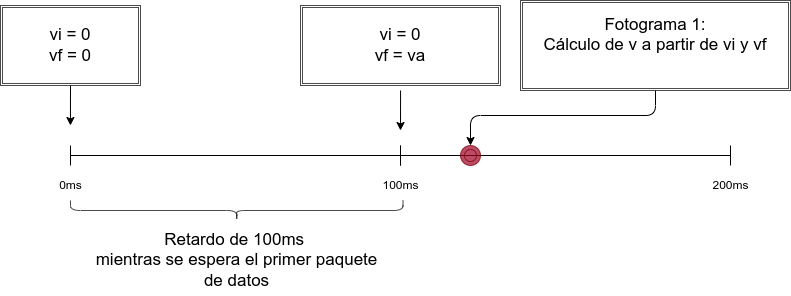
\includegraphics[scale=0.4]{images/interpolation-algorithm.png}
    \caption{Funcionamiento del algoritmo en los primeros 200ms}
    \label{fig: interpolation-algorithm}
\end{figure}

\begin{center}
\begin{minipage}{0.8\textwidth}
\begin{lstlisting}[language=c, label={code: interpolation}, caption={Controlador de movimiento}]
delta += Time.deltaTime;
 
if(delta > 0.001f) {
    delta = 0;
    finalSpeed = newSpeed;
    initialSpeed = finalSpeed;
}

currentSpeed = Mathf.Lerp( 
    initialSpeed, 
    finalSpeed, 
    delta
);

transform.Translate(currentSpeed * Time.deltaTime);
\end{lstlisting}
\end{minipage}
\end{center}


\subsubthesischapter{Modalidad Ligero}
La modalidad ligero, basada en el entrenamiento del tren inferior, se presenta como el primer escenario de juego. En esta modalidad, los parámetros de distancia o tiempo, seleccionados en el menú de configuración de la rutina, sirven como los pilares fundamentales del entrenamiento.

Como muestra la figura~\ref{fig: game-world}a la lógica subyacente del juego en dicha modalidad es la siguiente: al inicio, los usuarios establecen el valor de la distancia o el tiempo en el menú de configuración de las rutinas. Estos valores se utilizan como criterios para mejorar las estadísticas del jugador durante el juego. Por ejemplo, si se establece una distancia de 10 metros, el objetivo del jugador será completar esta distancia en el menor tiempo posible. De manera similar, si se elige un tiempo de 3 minutos, el objetivo será recorrer la mayor distancia posible dentro de ese límite temporal.

Para implementar esta lógica, fue necesario crear un terreno virtual que se reconstruye dinámicamente según la posición actual del jugador. Esto asegura que el jugador permanezca dentro del área de juego y evita que se pierda la coherencia del juego. Al finalizar cada rutina de rehabilitación en esta modalidad, las estadísticas del jugador son actualizadas para reflejar su desempeño, lo que proporciona una retroalimentación valiosa para su progreso.

\subsubthesischapter{Modalidad Clínico}
La modalidad clínico de nuestro juego serio representa una innovación significativa en nuestra aproximación terapéutica. Además de las características previamente mencionadas, esta modalidad integra los valores de la señal IEMG (Electromiografía de Superficie) capturados por nuestro pedal motorizado. Esta señal se convierte en un componente fundamental para establecer los desafíos en la escena del juego de esta modalidad.

Como muestra la figura~\ref{fig: game-world}b en esta modalidad clínica, se definen tres puntos clave en el recorrido hacia la meta. En cada uno de estos puntos, el juego verifica la media aritmética de los niveles de MCV capturados. Estos niveles se comparan con los valores de referencia predefinidos que se establecieron durante la fase de calibración y configuración del juego. Si la media de los niveles de MCV en un punto dado cumple con los requisitos establecidos, el jugador supera el reto asociado a ese punto y avanza en el juego.

\begin{figure}[ht]
    \centering
    \subfigure[Modalidad Ligero]{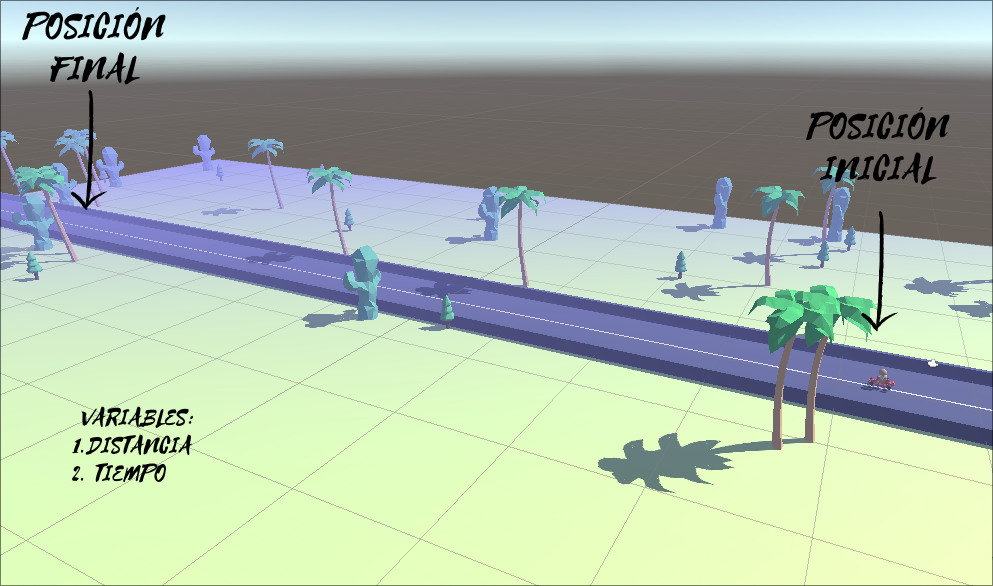
\includegraphics[height=5.2cm, width=0.45\textwidth]{images/game-world-1.png}}
    \subfigure[Modalidad Clínico]{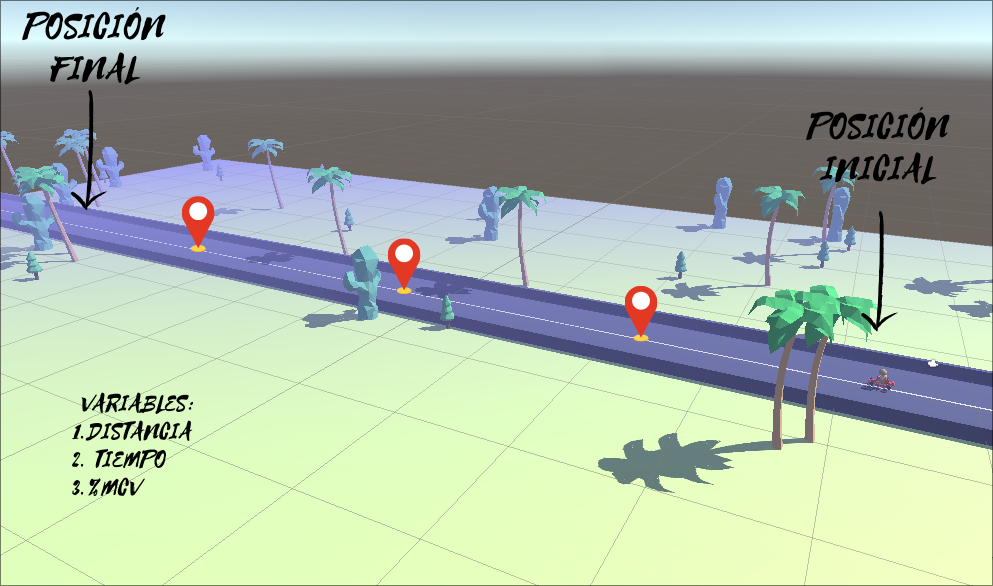
\includegraphics[height=5.2cm, width=0.45\textwidth]{images/game-world-2.png}}

    \caption{Modalidades del juego serio}
    \label{fig: game-world}
\end{figure}
    